In diesem Abschnitt wird die Variante des Deep Cascade Networks vorgestellt. Bei dieser Architektur handelt es sich um ein einzelnes neuronales 
Netzwerk, das schrittweise – also iterativ – während des Trainingsprozesses aufgebaut wird. Trotz der sukzessiven Erweiterung bleibt das Modell 
stets eine zusammenhängende Netzwerkstruktur. Zu Beginn des Trainings werden grundlegende Trainingsparameter festgelegt, insbesondere der 
verwendete Optimierungsalgorithmus sowie die Verlustfunktion, die für alle nachfolgenden Kaskadenstufen konsistent 
angewendet werden.

\begin{figure}[htpb]
    \centering
    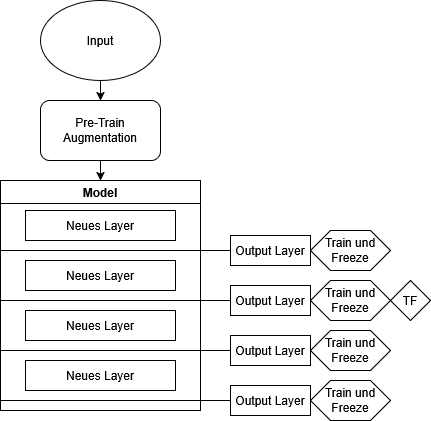
\includegraphics[height=10cm]{../../Graphiken/deepcascade_2.png}
    \caption{\label{fig:deepcascade}
    \small{In der Darstellung wird der Aufbau und Trainingsprozess von Deep Cascade Netzwerken veranschaulicht. Das zugrunde liegende Modell 
    besteht aus mehreren Schichten (Layern), die sukzessive – also nacheinander – trainiert werden. Zur Unterstützung des schrittweisen 
    Trainingsprozesses werden temporäre Output-Layer extern am Netzwerk angebracht. Diese dienen ausschließlich dem Training 
    des jeweils aktuellen Abschnitts und werden nach dessen Abschluss entfernt, da ihre Integration in die Hauptstruktur des Netzwerks den 
    internen Informationsfluss beeinträchtigen würde. Nach dem Training werden alle bisherigen Layer eingefroren. TF kann zwischen jedem Layer 
    vollzogen werden.}}
\end{figure}

Nachdem sowohl der Optimierer als auch die Verlustfunktion festgelegt wurden, beginnt der schrittweise Aufbau des Deep Cascade Netzwerks mit der 
Definition der ersten Netzwerkschicht. Diese wird zunächst durch eine temporäre Ausgabeschicht (Output-Layer) ergänzt und anschließend trainiert. 
Nach Abschluss des Trainings wird der Output-Layer entfernt und die trainierte Schicht eingefroren, sodass ihre Gewichtungen im weiteren 
Trainingsverlauf nicht mehr angepasst werden. Danach wird eine neue Schicht dem Netzwerk hinzugefügt, wie in Abbildung 
\ref{fig:deepcascade} dargestellt.

Dieser Zyklus aus Training, Entfernen des Output-Layers, Einfrieren der trainierten Schicht und Hinzufügen einer weiteren Schicht wiederholt sich 
iterativ. Optional kann zu einem beliebigen Zeitpunkt TF initiiert werden, indem
anstelle des ursprünglichen Source-Datensatzes ein Target-Datensatz für das Training verwendet wird.
